\documentclass[11pt,a4paper]{article}
\usepackage{settings}
%<---------------------------------------------------------------------------->%
\title{\textsc{Kelighine} 遊戲說明}
\author{陳\ 捷\thanks{\ 一個極其無聊的人。聯絡方式:\href{https://jessekelighine.com}{\texttt{jessekelighine.com}}}}
\date{2020 年 2 月 \quad 版本 2.1\thanks{\ 最後更新時間: \today。更新紀錄參見表\ \ref{update}。}}
%<---------------------------------------------------------------------------->%

\begin{document}

\maketitle

\section{遊戲介紹} %% section 1

Kelighine 是在我國中時(2011 或 2012 年)不經意發明出來的一款遊戲。
	\footnote{\ 其實這個遊戲一直以來都沒有名字,至少我沒有印象。
	Kelighine 這個名字是我猜想國中的我會幫這個遊戲起的名字。}
原本只是畫出了這個奇怪的圖,
	\footnote{\ 參見圖 \ref{a}。}
後來因為上課太無聊所以用這個壓在桌墊下的圖當作「棋盤」,
逐漸的發想出一個遊戲。
Kelighine 基本上是一個類似 Snakes and Ladders 的運氣遊戲,
畢竟自己一個人上課也只能擲擲骰子跟自己玩,沒有太多玩家自己的選擇。
又因為這個遊戲是在國中時逐步發想的,
所以規則大多都沒有確定,也存在過很多不同的玩法,
但是有些基本的規則跟\underdot{精神}是一樣的。
因此我給了兩版規則:
\begin{itemize}
	\item 版本一是最原始的規則,也是我印象中最早也最簡單的規則。
	\item 版本二是改良的規則,增加玩家一點點主觀能動性,其實沒有差很多。
\end{itemize}
這麼做的目的一方面當然是想要給玩家一些選擇,
但另一方面也是想要記錄下這遊戲最原始的樣子。
其實在了解規則後,玩家會發現 Kelighine 可以很容易的在版本一下擴充,版本二就是版本一的擴充。
會這麼寫也是因為這是我國中時很常做的事,每次玩的時候都會加一些突然想到的規則,
但是很多都加得莫名奇妙(像是我記得曾經出現過飛彈的設定…)。
所以版本二是 2020 年的我認為不失遊戲精神又增加一點點挑戰性的擴充規則。

本文第 \ref{SECTION_TWO} 節中將說說明遊戲規則:前半段說明基本遊戲規則,後半段說明兩種玩法;
第 \ref{SECTION_THREE} 節為後記;
圖表附於文末。

\section{遊戲規則} \label{SECTION_TWO}%% section 2

正如介紹中所說, Kelighine 有一些不變的精神,
所以接下來 \ref{board_intro}、 \ref{moving} 及 \ref{push} 小節介紹基本精神,
最後 \ref{ver1} 和 \ref{ver2} 小節給出兩種規則。
	\footnote{\ 本說明說使用方法:按照順序讀完遊戲規則這節,
	並且在用遊戲規則版本二玩之前先至少玩過一次 \ref{ver1} 節版本一遊戲規則。}

\subsection{棋盤介紹} \label{board_intro} %% section 2.1

圖 \ref{a} 是原始棋盤,但是為了方便起見,
以下遊戲說明請搭配圖 \ref{b}。
而圖 \ref{b} 中的 A1 對應到圖 \ref{a} 中的羅馬數字 I。
\begin{enumerate}
	\item
		每個編號對應到一個棋子可以放置的位置(稱為格),
		而每個編號中有數字的格可以分成黑白兩類:
		數字為奇數的為白格,數字為偶數的為黑格。沒有數字編號的(只有羅馬字母的)則沒有分類。
	\item
		棋盤由格的編號之首字母主要分為三階: A 階、B 階、C 階。
		A 階有 16 格,B 階有 8 格,C 階有 8 格。
	\item
		兩格相鄰指的是兩格邊相鄰。\\
		\zB B7 與 A14、A13、C6、C7 相鄰。
		A13 與 A14、A12、B7、G 相鄰,但不與 B6 相鄰。
		特別地, I 與 A2、A3 相鄰,K、H、L 以此類推。
\end{enumerate}

\subsection{基本走法} \label{moving} %% section 2.2

\begin{enumerate}
	\item \label{clock}
		玩家依序擲骰,由點數決定棋子前進幾格,
		在同一階中依逆時針方向移動棋子。
			\footnote{\ 逆時針方向移動的規則在遊戲規則版本二中會有例外,
			詳見小節 \ref{ver2} 中的規則。}\\
		\zB 若一棋子位置在 A3 而該輪玩家擲到 4,則前進到 A7。
		類似地,若一棋子位置在 C3 而該輪玩家擲到 4,則前進到 C7。
	\item \label{initial}
		每個棋子初始位置在 H、I、K、L 其中一格。
		遊戲開始時則依照擲骰結果進入 A 階中的對應位置。\\
		\zB 若一棋子初始位置在 I 且擲到 2,則前進到 A4。若擲到 1,前進到 A3。
	\item \label{3}
		若一個棋子繞行完一階(至少回到原本進入該階的位置),
		則該棋子獲得進入下一階的資格。\\
		\zB 若一棋子初始位置在 I 並且已經繞行 A 階一圈
		(走回 A3 以後,包含 A3)並且現在位置在 A5,
			\footnote{\ A 階較特殊,因為棋子在 A 階其實沒有明確進入位置,
			所以在 A 階判定是否繞行完一圈的起始點是初始位置相鄰兩個 A 階的格中編號數字較大者。\\
			\zB 初始位置 H 的棋子要至少走回 A11 才算繞行完成。}
		則在擲骰後可以決定要繼續在 A 階中繞行或進入下一階。
		(詳見 \ref{next}.\! 擲骰)
	\item \label{next}
		\textsf{擲骰}:
		每輪玩家可以在擲骰後選擇\underdot{使用擲出點數}在同一階繼續移動或\underdot{放棄擲骰}進入下一階。
			\footnote{\ \underdot{放棄擲骰}指的不是不丟骰子,而是擲出後可以選擇不使用骰子點數。}
		(後者的選擇稱為\underdot{晉升})
		進入下一階的格(稱為進入點)只能是與現在所在格相鄰的格。\\
		\zB 若當一個棋子從 B2 進入 B 階並且繞行完 B 階並且停在 B2,
		可以在擲骰後選擇繼續繞行 B 階或晉升到 C 階的 C1 或 C2,此二格都與 B2 相鄰。
	\item
		若棋子位在 D、E、F、G 之一,則擲骰後走法與遊戲開始時走法相同,
		不用放棄擲骰。亦即,從 D、E、F、G 不用晉升,使用擲出點數即可走到 A 階。\\
		% \footnote{\ 將在小節 \ref{push} 中解釋棋子如何會落到 D、E、F、G 這四個位置。}\\
		\zB 若一棋子在 E 並且擲到 2,則該棋移動到 A6。
	\item
		\textsf{目標}:玩家試圖讓自己的棋子從初始位置移動到 J 結束位置。\\
		\zB 若一棋子繞行完 C 階便可以晉升到 J 並且將該棋從棋盤取下。
\end{enumerate}

\subsection{排擠} \label{push} %% section 2.3

排擠是基本走法的限制條件,也是 Kelighine 中最重要的規則。
其中 \ref{basic}.\! 是原則;
\ref{rules}.\! 是排擠的規則,是除了擲骰及晉升以外棋子移動的唯一方式;
\ref{direct}.\! 和 \ref{indirect}.\! 是觸發排擠的兩種方式;
\ref{order}.、\ref{passive}.\! 和 \ref{conti}.\! 是如果同時觸發多個排擠時的執行順序以及效力大小;
\ref{add}.\! 是在排擠被觸發的情況下繞行的認定。

\begin{enumerate}
	\item \label{basic}
		一格中不可以同時有兩個棋子。
	\item \label{rules}
		\textsf{排擠規則}:
		\begin{enumerate}
			\item 若一棋子在 A 階被排擠,該棋子移動到 D、E、F、G 中距離最近的一格。
			\item 
				若一棋子在 B(或 C)階被排擠,
				則該棋子下移一階到 A(或 B)階中與原所在格相鄰的兩格之一,
				而被排擠棋子的持有玩家可以選擇到哪一格。
			\item
				若被排擠的棋子無法依照上述規則移動,
				則移動到 D、E、F、G 中距離最近的格之一,
				被排擠棋子的持有玩家可以選擇到哪一格。\\
				\zB 若上一棋子在 A5 且已經有另一棋子在 A6,則移動到 B3 的棋子可以被排擠到 E。
					\footnote{\ 這是 \ref{indirect}.\! 間接排擠的例子。}
			\item
				若被排擠的棋子無法依照上述規則移動,則該棋子回到\underdot{初始位置}且繞行進度歸零。
					\footnote{\ 這條在小節 \ref{ver2} 遊戲規則版本二中才適用。}
		\end{enumerate}
	\item \label{direct}
		\textsf{直接排擠}:
		若一棋子移動到有另一棋子所在的一格時,原本在該格的棋子依照排擠規則排擠。
		特別地,晉升移動到下一階的選擇不可以直接排擠棋子。\\
		\zB 若原本有一棋子在 A2 並且另一個棋子剛好要移動到該格,
		則原本在該格的棋子要移動到 D。
		類似地,若原本有一棋子在 C1 並且另一個棋子剛好要移動到該格,
		則由原本在該格棋子的持有玩家選擇該棋子要移動到 B1 或 B2。
		特別地,若有一已經繞行完 A 階的棋子 a 在 A4 並且另一棋子 b 在 B2,
		則 a 不可以晉升。
	\item \label{indirect}
		\textsf{間接排擠}:上一個棋子
			\footnote{\ \label{last}
			上一個棋子指的是\underdot{上一位玩家}移動或被移動的\underdot{最後一個}棋子。\\
			\zB 假設在遊戲規則版本一下有四個玩家,而玩家四在他那輪直接排擠玩家二的棋子,
			則雖然玩家二的棋子是最後一個移動的棋子,但是對於下一位玩家(玩家一)來說,
			玩家四才是上一位玩家,所以決定玩家一這輪的間接效果是玩家四的棋子。\\
			\zB 假設在遊戲版本二下,玩家二在最後一部動作直接排擠掉自己的棋子,
			則決定下一輪有間接效果的棋子是該被直接排擠的棋子,
			而非造成直接排擠的棋子。}
		a 所在之格會決定一些其他格 (由以下列點表述)
		使得若下一個被移動的棋子 b 移動到這些格上,
		則 b 依照排擠規則排擠。
			\footnote{\ 下一個棋子指的是這輪中移動的棋子
			(如果在遊戲規則版本二下則是這輪中\underdot{所有}棋子),
			縱使上一個棋子 a 在這輪中被排擠,有間接效果的格子不變。
			詳細排擠流程請參見表 \ref{order_one} 及 \ref{order_two}。}
		這些可以間接排擠棋子的格子稱為有\underdot{間接排擠效果}。
		\begin{enumerate}
			\item
				若上一個棋子 a 在 A 階的 A$m$ 格上,
				則在 A 階中從 A$m$ 逆時針數的第 4、8 及 12 個(3 個)與 B、C 階中和 A$m$
				顏色相同的所有格(8 個)有間接排擠效果。\\
				\zB 若上一個棋子 a 移動到 A5,
				則 A1、A9、A13(A 階中與 A5 組成十字架對應到的格)、
				B1、B3、B5、B7、C1、C3、C5、C7(B、C 階中跟 A5 顏色相同的格)
				共 11 格有間接排擠效果。 亦即,
				而下一個棋子 b 若移動到這 11 格任一格上, b 就要被排擠;
				假設 b 是移動到 B1,b 就要被排擠到 A1 或 A2;
				假設 b 是移動到 A9,b 就要被排擠到 F。
			\item
				若上一個棋子 a 在 B 階的 B$m$ 格上,
				則在 B、C 階中和 B$m$ 顏色相同、不含 B$m$ 本身的所有格(7 個)有間接排擠效果。
			\item
				若上一個棋子 a 在 C 階的 C$m$ 格上,
				則在 C 階中和 C$m$ 顏色相同、不含 C$m$ 本身的所有格(3 個)有間接排擠效果。
		\end{enumerate}
	\item \label{order}
		直接排擠適用先於間接排擠。
			\footnote{\ 參見表 \ref{order_one} 及 \ref{order_two} 中每輪動作執行順序中排擠順序。}\\
		\zB 若一棋子 a 從 B2 移動到 B3,而 B3 有間接排擠效果並且在上有一棋子 b,
		則 a 先直接排擠 b 並且確認需不需要再次被排擠直到 b 停止移動,
		再考慮 B3 對 a 的間接排擠效果。
	\item \label{passive}
		\textsf{被動性}:
		被排擠的棋子不可以直接排擠其他棋子。\\
		\zB 若上一棋子在 A5 且下一棋子 b 移動到 B3, b 不可被排擠到 A5。
	\item \label{conti}
		\textsf{持續性}:
		被排擠的棋子若被排擠到有間接排擠效果的格子上,
		則須再次受間接效果影響,直到該棋子無法繼續被排擠為止。\\
		\zB 若上一棋子 a 在 A7 且下一棋子 b 移動到 C3,則若 b 被排擠到 B3,
		b 須再次被間接排擠到 A6 或 A5。
	\item \label{add}
		基本走法 \ref{3}.\! 在排擠下的補充規則:
		\begin{enumerate}
			\item
				排擠不影響已經完成的繞行。\\
				\zB 若一棋子已經完成繞行 B 階,但是被排擠到 D,
				則該棋子無需再次繞行 B 階便可進入 C 階。
			\item
				若一棋子在走到超過進入點時被排擠,則視為完成繞行該層。\\
				\zB 若一棋子之 B 層進入點為 B6 並且現在位置在 B5 ,
				假設擲到 2 走到 B7 時被排擠到 A13,則該棋視為繞行完 B 層,
				亦即該棋獲得進入 C 階的資格。
			\item
				若一棋子在繞行 A 階時被排擠,繞行的進度不受影響。\\
				\zB 若一棋子的初始位置為 I,無論途中有沒有被排擠到 D、E、F、G,
				只要至少走超過 A3 就算是繞行完成。
			\item
				若一棋子在繞行 B 或 C 階中被排擠,則繞行進度從下次再進入該層的進入點重新計算。\\
				\zB 若一棋子由 C8 進入 C 階並且在走到 C3 時被排擠到 B4,
				則繞行進度歸零,由下次再進入 C 層時的進入點重新計算。
		\end{enumerate}
\end{enumerate}

\subsection{遊戲規則版本一} \label{ver1} %% section 2.4

\begin{enumerate}
	\item 玩家數: 2 到 4 人。
	\item
		需要用具:
		\begin{itemize}
			\item 棋盤 1 個。
			\item 四面骰或六面骰 1 個:作為骰子使用。
			\item 一塊錢銅板 2 到 4 個:以記錄各階進入點,一個玩家一個銅板。
				\footnote{\ 建議可以用年份不同的一塊錢,這樣才分得出哪個是誰的。}
			\item 長相不同的六面骰 2 到 4 個:作為棋子使用,一個玩家一個六面骰作為棋子。
		\end{itemize}
	\item
		在我印象中,傳統上,初始位置是玩家一在 I,玩家二在 H,玩家三在 K,玩家四在 L,
		並且由玩家一先骰。擲骰順序按照玩家編號或順、逆時針輪轉皆可。
	\item \label{facing}
		每位玩家一開始的棋子都是 6 點的面朝上。
		繞行完 A 階則將該棋子轉為 1 點的面朝上,
		繞行完 B 階則 2 點的面朝上,
		繞行完 C 階則 3 點的面朝上。
	\item \label{coin}
		在進入尚未繞行完成的一階時,將銅板置於進入點上,
		繞行完成後取下。
		特別地,由於 A 階的進入點固定,所以繞行 A 階時不用放銅板。
	\item
		先走到 J 的玩家獲勝。
			\footnote{\ 參見表 \ref{order_one} 每輪動作執行順序中的版本一幫助遊戲進行。}
\end{enumerate}

\subsection{遊戲規則版本二} \label{ver2} %% section 2.5

\begin{enumerate}
	\item 玩家數: 2 人。
	\item
		需要用具:
		\begin{itemize}
			\item 棋盤 1 個。
			\item 四面骰 2 個:作為骰子使用。
			\item 十塊錢銅板 1 個:記錄上一棋子的位置。
			\item 一塊錢銅板 4 個:用以記錄各階進入點,一個玩家兩個銅板。
			\item 兩種長相不同的六面骰各 3 個共 6 個:作為棋子使用,一個玩家 3 個相同的六面骰作為棋子。
		\end{itemize}
	\item
		玩家一的初始位置在 I,玩家二在 H,並且由玩家一先骰。
	\item
		記錄方式與小節 \ref{ver1} 中的第 \ref{facing} 及 \ref{coin} 點相同。
		因為現在每個玩家有三個棋子,所以為了避免忘記,以一個十塊錢銅板記錄\underdot{上一個棋子}。
			\footnote{\ 參見註釋 \ref{last}。}
	\item
		新增規則:
			\footnote{\ 表 \ref{order_two} 為每輪動作順序表準。}
		\begin{enumerate}
			\item
				所有原本表述的規則除非有特別說明例外,則仍然成立。
			\item 
				\textsf{遊戲目標}:先將自己的三個棋子都送到 J 的玩家獲勝。
			\item
				\textsf{棋子上場}:同個玩家的棋子的初始位置相同。
				遊戲開始時兩位玩家各有一棋子在各自的初始位置,
				並且上場方式同小節 \ref{moving} 中第 \ref{initial}。
				剩餘棋子在\underdot{場下}位置,
				而每當玩家擲到\underdot{兩個相同點數}或場上\underdot{沒有自己的棋子}時,
				則得在擲色前移動一個原本在場下的棋子到各自的初始位置。\\
				\zB 若玩家一有一棋子 a 在場上,兩個在場下,並且擲到 2 個 2,
				則玩家一可以先把一個場下的棋子 b 移動到初始位置 I 並讓 b 走到 A4,
				再讓 a 走 2 步。
			\item
				\textsf{棋子行走}(\ref{moving} 基本走法第 \ref{clock} 的例外):
				若一棋子\underdot{完成繞行}某階,則玩家得選擇讓該棋子可以在該階正或逆時針移動。
				亦即,點數 1 朝上的棋子可以在 A 階中任意方向移動;
				點數 2 朝上的棋子可以在 B 階中任意方向移動;
				點數 3 朝上的棋子可以在 C 階中任意方向移動。\\
				\zB 若有一數 1 朝上的棋子位在 A15 且玩家骰到其中一個點數為 1,
				則該棋子得移動到 A14 或 A16。
			\item \label{ok}
				\textsf{擲骰}:
				\begin{enumerate}
					\item
						每輪玩家同時擲 2 個骰子,
						玩家可以選擇將 2 個點數\underdot{拆開使用}在不同的 2 個棋子上或用在同一個棋子上,
						但是不可拆分同個骰子上的點數。\\
						\zB 假設玩家一有一個棋子 a 在 A4(完成繞行 A 階),
						一個棋子 b 在 B3(正在繞行 B 階,進入點在 B4),
						另一棋子 c 在場下。若該玩家擲到 1 跟 3,則該玩家可以先使 b 移動到 B4 完成繞行,
						再放棄另一個骰子的點數讓 a 晉升到 B 階;
						或是可以先使 b 移動到 B4 完成繞行,再使 b 移動到 C3。
						但是不能將擲到的 3 點拆分成
						2 點及 1 點分配給兩個棋子或把擲到的 $3+1$ 點分成 2 個 2 點給同一個棋子使用。
							\footnote{\ 如此規定意旨是若本例子中的 B4 有間接排擠效果,則 b 移動到 B4 時要先受排擠。}
					\item
						如果玩家擲到 2 個 1 點,玩家可以有三種選擇:
						(1) 視為有 4 個 1 點可以使用 (2) 重新擲骰 (3) 仍視為擲到 2 個 1 點。
					\item
						若其中一位玩家在場上只剩下 1 個棋子(其他棋子都已經走到 J),
						該玩家得選擇擲出的 2 個點數之一使用,另一個放棄使用。
					\item
						玩家執行完 2 個骰子的效果後則該輪結束。
				\end{enumerate}
			\item
				每個棋子的繞行進度各自獨立(進入下一階的資格各自獨立)。
			\item
				B 階(C 階)同時至多只能有一個自己的棋子正在繞行,
				亦即,每階只能有一個自己的一塊錢。\\
				\zB 假設玩家一有一個棋子 a 在 A4(完成繞行),一個棋子 b 在 B3(正在繞行,進入點在 B4),
				另一棋子 c 未上場。若該玩家擲到 1 跟 3,玩家不能直接讓 a 晉升到 B 階,
				因為此時 B 階會出現\underdot{兩個}玩家一的銅板。
			\item
				一個玩家只有 2 個一塊錢銅板,亦即整個棋盤最多只能同時記錄兩個進入點。
					\footnote{\ 一塊銅板的作用不只是作為繞行進入點的紀錄,也作為限制玩家的條件。
					但是注意到 A 階不用銅板,所以可以同時有多個棋子繞行 A 階。}\\
				\zB 假設玩家一有一個棋子 a 在 B4(正在繞行),一個棋子 b 在 C3(正在繞行),
				另一棋子 c 未上場。若玩家擲到 1 跟 3,玩家不能直接讓 c 走上場,
				因為該玩家已經\underdot{沒有銅板}了。
			\item
				排擠規則對於所有棋子(包含自己的棋子)都適用。
				一輪內排擠的執行順序依照表 \ref{order_two} 中決定。
		\end{enumerate}
\end{enumerate}

\section{後記} \label{SECTION_THREE} %% section 3

\begin{quote}
	這張圖(應該)是國中的時候畫的,而這個想法是小學的時候就有了,
	也畫過很多不同的版本,但是至於是怎麼想出來的就不可考了,
	可以猜想的應該是看到曼陀羅之類的東西吧?我倒是記得很清楚畫出來之後我一直壓在國中的桌墊下,
	然後因為上課太無聊,又鉛筆盒裡面有骰子,就想出了一個可以把這張圖當作棋盤的遊戲。
	\\\indent
	其實原圖在國中畢業的時候就遺失了,現在只剩下我之前影印的一張。
	剛剛才發現剛好的是,我是在去年生日的時候把影印的那張拍照下來,用影像描圖簡單的電子化。
		\footnote{\ 參見圖 \ref{c}。}
	然後前幾天不知道發什麼神經(太無聊吧?)想說一直都有想要重新畫一張精緻版的,
	畢竟國中的時候以為自己是希臘人尺規作圖又經過風吹日曬看起來有點殘破,
	所以這幾天就每天花一點時間重畫,其中今天花了最多時間。
	歷經一年終於成功的電子重製,結果蠻滿意的,很有成就感 哈哈。
		\footnote{\ 重製版便是圖 \ref{a}。}
\end{quote}

\noindent
這兩段是貳〇貳〇年貳月拾日發的 Instagram 文節錄,而之所以想把遊戲完整地寫下來,
就是因為有個高中同學問我要怎麼玩,所以我就想說把它寫下來也是不錯,
反正閒閒沒事做,所以隔天就大致生出來了。

以紀錄的角度來看的話我的工作已經完成了,
但是我還是有另外一個小小的希望:
就是真的把一個棋盤做出來,用木頭或竹子之類的,
同時也做出專用的「銅板」跟「骰子」,
畢竟我之所以選的用具都是唾手可得的東西,
就是因為國中的我也只有鉛筆盒裡面的東西…,
另一方面也是因為我希望這個遊戲是只要一張紙印出來就可以玩。
但是作為遊戲的發明者,能在客廳正中間擺上一個長得莫名其妙神秘學的棋盤也是滿帥的啦,哈哈哈。
如果有人有 CNC 或是雷射切割器之類的然後也覺得這個遊戲不錯,
拜託拜託跟我講,我可以提供 AI 檔,
然後付錢把它做出來…吧(拜託不要太貴我就願意…)。

最後,因為這些規則是我國中想出來的,
又是在很多年後的今天在沒有試玩幾次的情況下就寫下來的,
所以很有可能有不清楚或甚至自相矛盾、無法解決之處。
如果有發現的話 (我猜錯字也很多…),
請不要吝嗇於通知我~~\\

\vfill\centerline{***\ \ 正文結束 後頁為附圖及附表\ \ ***}\vfill %% end section
\pagebreak

\begin{table} 
	\caption{每輪動作執行順序版本一}
	\label{order_one}
	\centering
	\vspace{0.1cm}
	\begin{tabular}{cl}
		\toprule
			步驟 & 動作\\
		\midrule
			1 & 確認上一棋子的位置並找出有間接排擠效果的格子。\\
			2 & 擲骰,再確認可不可以晉升。\\
			  & 若晉升,則選擇上升一階的格,放置銅板,跳到第 6 步。\\
			3 & 移動棋子。\\
			4 & 確認移動棋子後是否完成該階繞行。\\
			  & 若完成,將棋子翻到對應的面,並且取下銅板。\\
			5 & 如果移動到的格已經有其他棋子 $\implies$ 執行直接排擠。\\
			  & 若被直接排擠的棋子被排擠到有間接效果的格子上\\
			  & $\implies$ 執行間接排擠直到停止。\\
			6 & 如果移動到的格有間接排擠效果 $\implies$ 執行間接排擠直到停止。\\
			7 & 本輪結束。\\
		\bottomrule
	\end{tabular}
\end{table}

\begin{table} 
	\caption{每輪動作執行順序版本二}
	\label{order_two}
	\centering
	\vspace{0.1cm}
	\begin{tabular}{cl}
		\toprule
			步驟 & 動作\\
		\midrule
			1 & 確認對手最後一棋子的位置,在上面放置十塊錢,\\
			  & 並找出有間接排擠效果的格子。\\
			2 & 擲骰。\\
			\midrule
			3 & 選擇使用的點數並移動棋子。(移動或晉升)\\
			  & 若選擇晉升 $\implies$ 選擇上升一階的格,放置一塊錢,跳到第 6 步。\\
			  & \textsf{注意}:同階不能有兩個自己的一塊錢。\\
			4 & 確認移動棋子後是否完成該階繞行。\\
			  & 若完成,將棋子翻到對應的面,並且取下一塊錢。\\
			5 & 如果移動到的格已經有其他棋子 $\implies$ 執行直接排擠。\\
			  & 若被直接排擠的棋子被排擠到有間接效果的格子上\\
			  & $\implies$ 執行間接排擠直到停止。\\
			6 & 如果移動到的格有間接排擠效果 $\implies$ 執行間接排擠直到停止。\\
			7 & 若仍有點數尚未用完,回到步驟 3。\\
			8 & 本輪結束。\\
		\bottomrule
	\end{tabular}
\end{table}

\begin{table} 
	\caption{更新紀錄}
	\label{update}
	\centering
	\vspace{0.1cm}
	\begin{tabular}{lcp{9cm}}
		\toprule
			版本 & 日期 & 內容 \\
		\midrule
			1.0.0 & \texttt{2020-02-11} & 初版。                           \\
			2.0.0 & \texttt{2020-02-13} & 遊戲規則版本二大幅修改。         \\
			2.1.0 & \texttt{2020-02-16} & 遊戲規則版本二棋子上場規則修正。 \\
			2.1.1 & \texttt{2020-02-27} & 錯字改正。                       \\
                  &                & 按:在自己玩過幾次之後發現在版本二的規則之
				  下還是有點(非常)無聊,所以我也沒辦法啦,只希望大家可以自己
				  擴充或跟很小的小朋友玩吧… \\
			2.1.2 & \texttt{2020-06-16} & 無聊過來改一下錯字跟字體。       \\
			2.1.3 & \texttt{2021-02-05} & 重新用 Xe\TeX\ 來排版。 \\
			2.1.4 & \texttt{2021-08-05} & 放到網站上、加上 roadmap。 \\
			2.1.4 & \texttt{2023-12-12} & 改聯絡方式。 \\
			2.1.4 & \texttt{2024-05-26} & 重新排版。 \\
		\bottomrule
	\end{tabular}
\end{table}

\begin{figure}
	\caption{棋盤}
	\label{a}
	\centerline{ 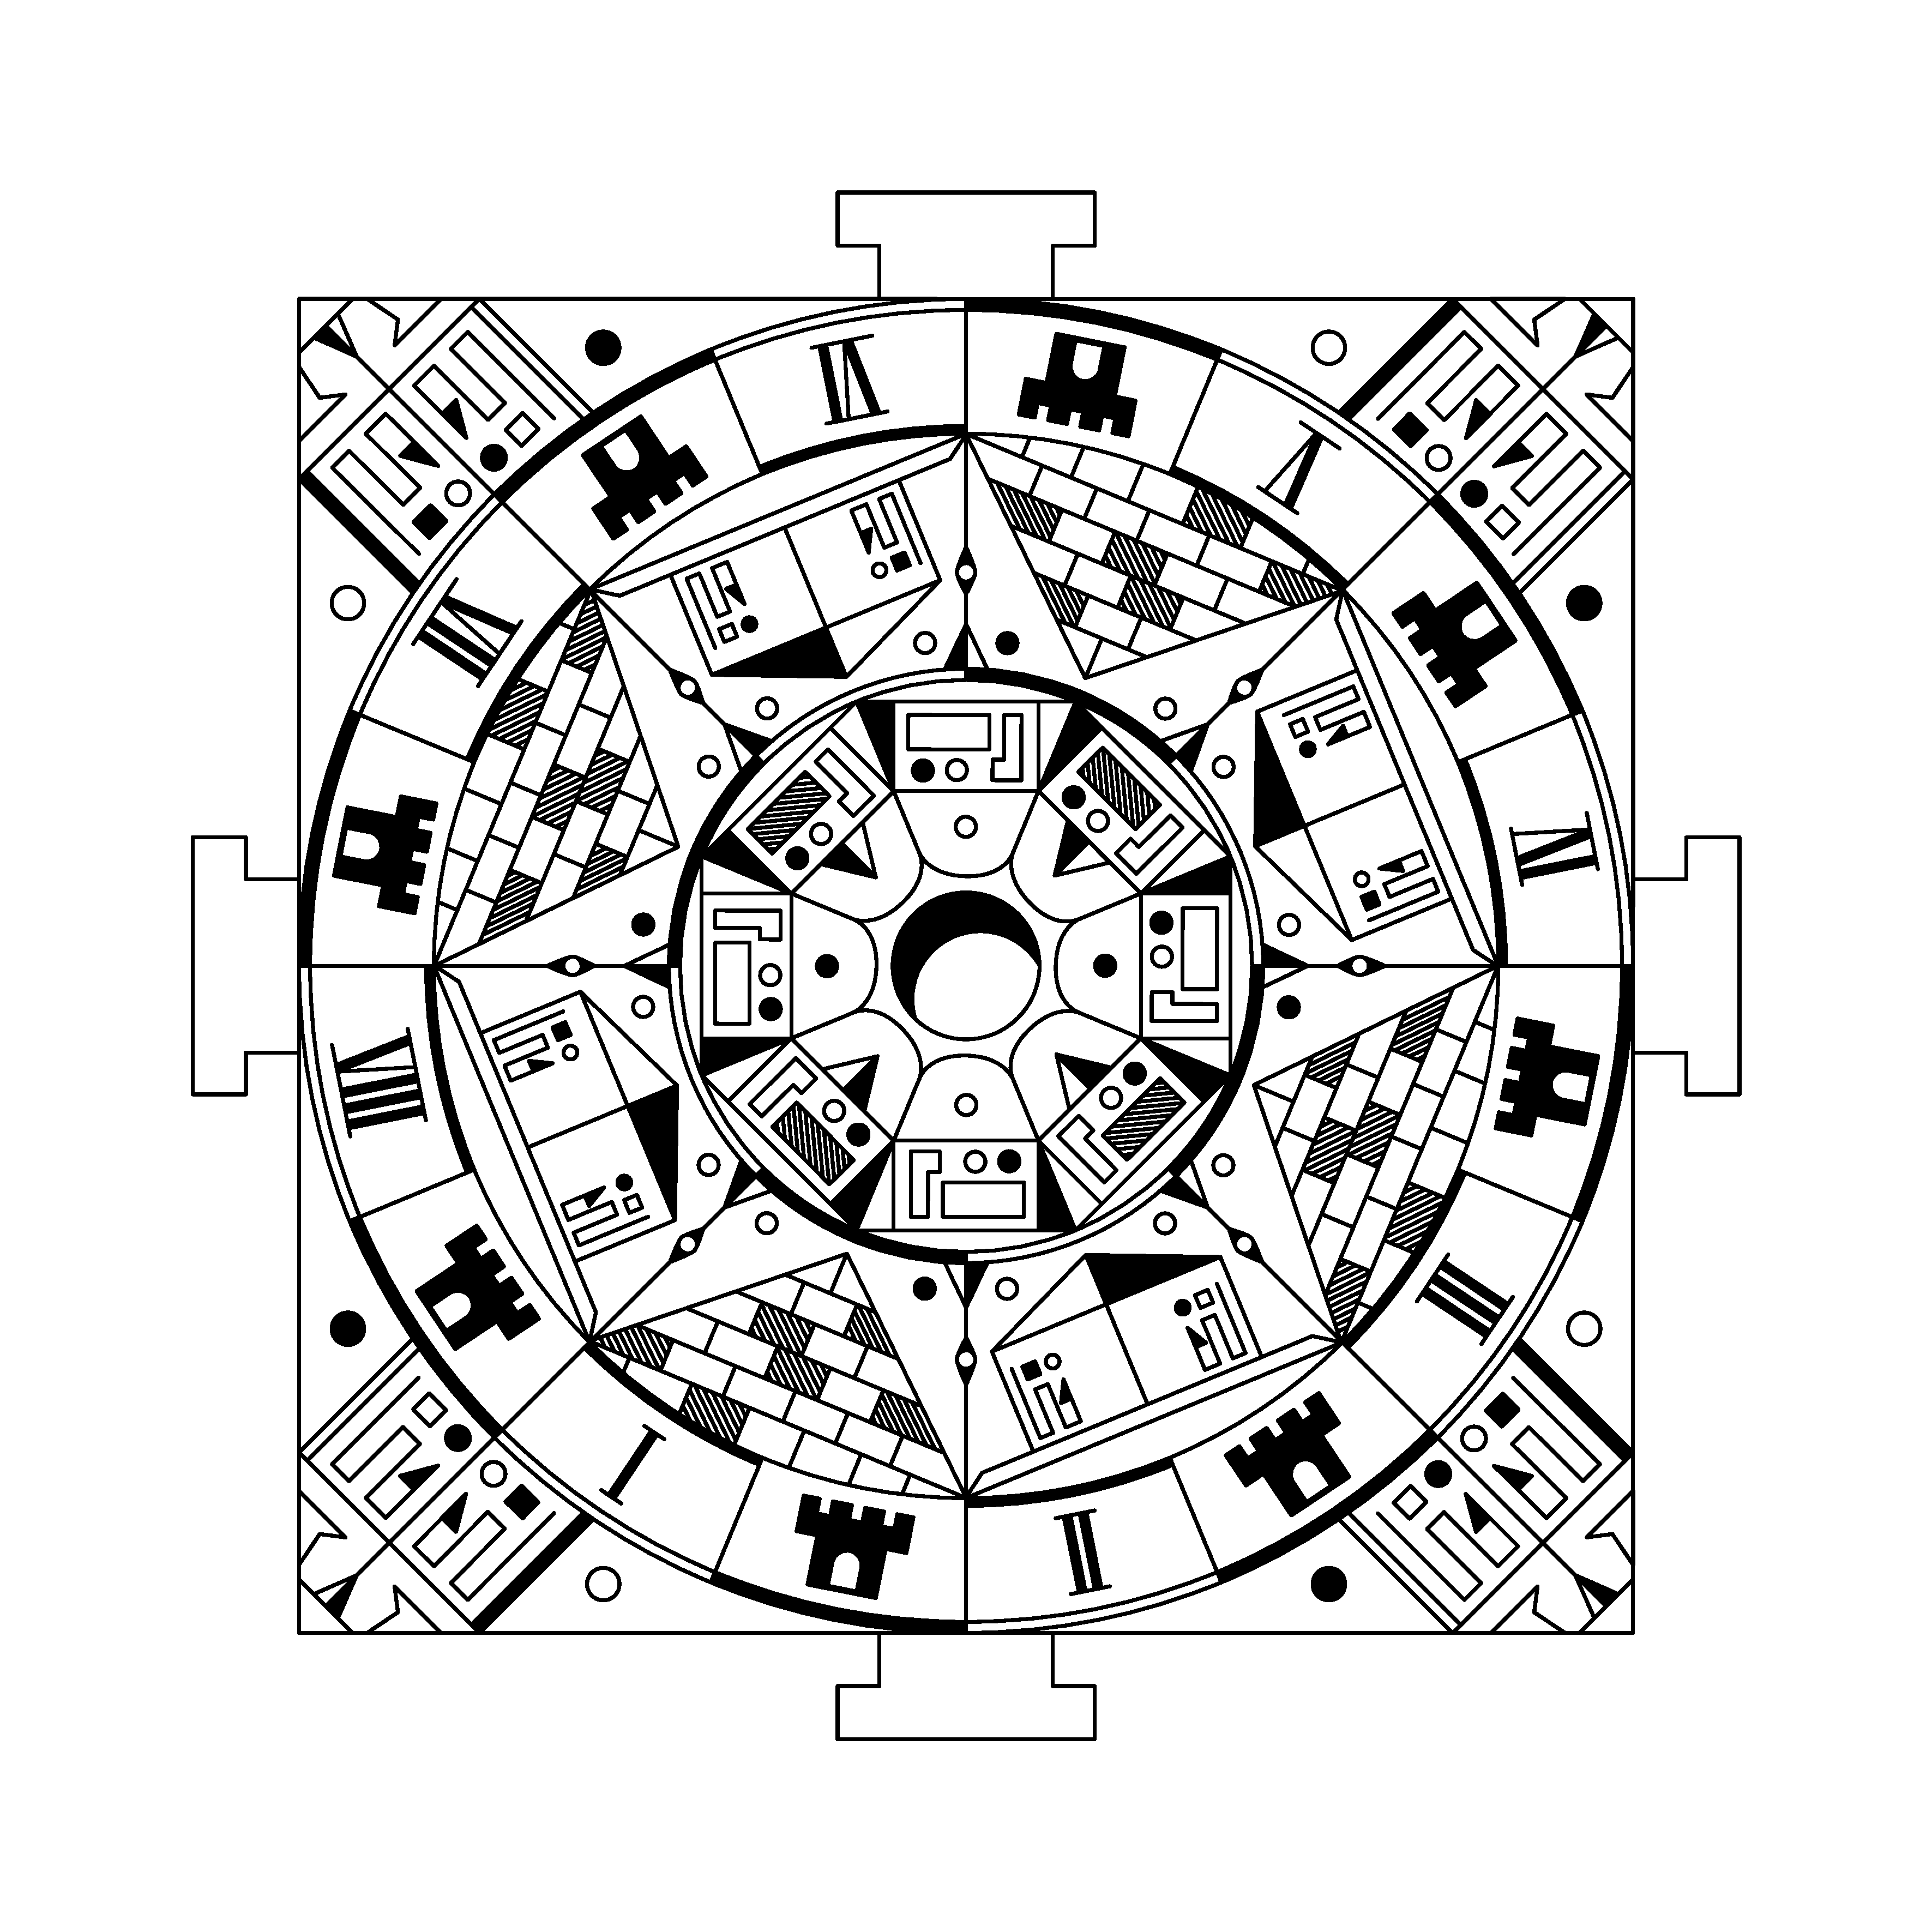
\includegraphics[scale = 0.4]{mandala-remastered} }
\end{figure}

\begin{figure}
	\caption{說明棋盤}
	\label{b}
	\centerline{ 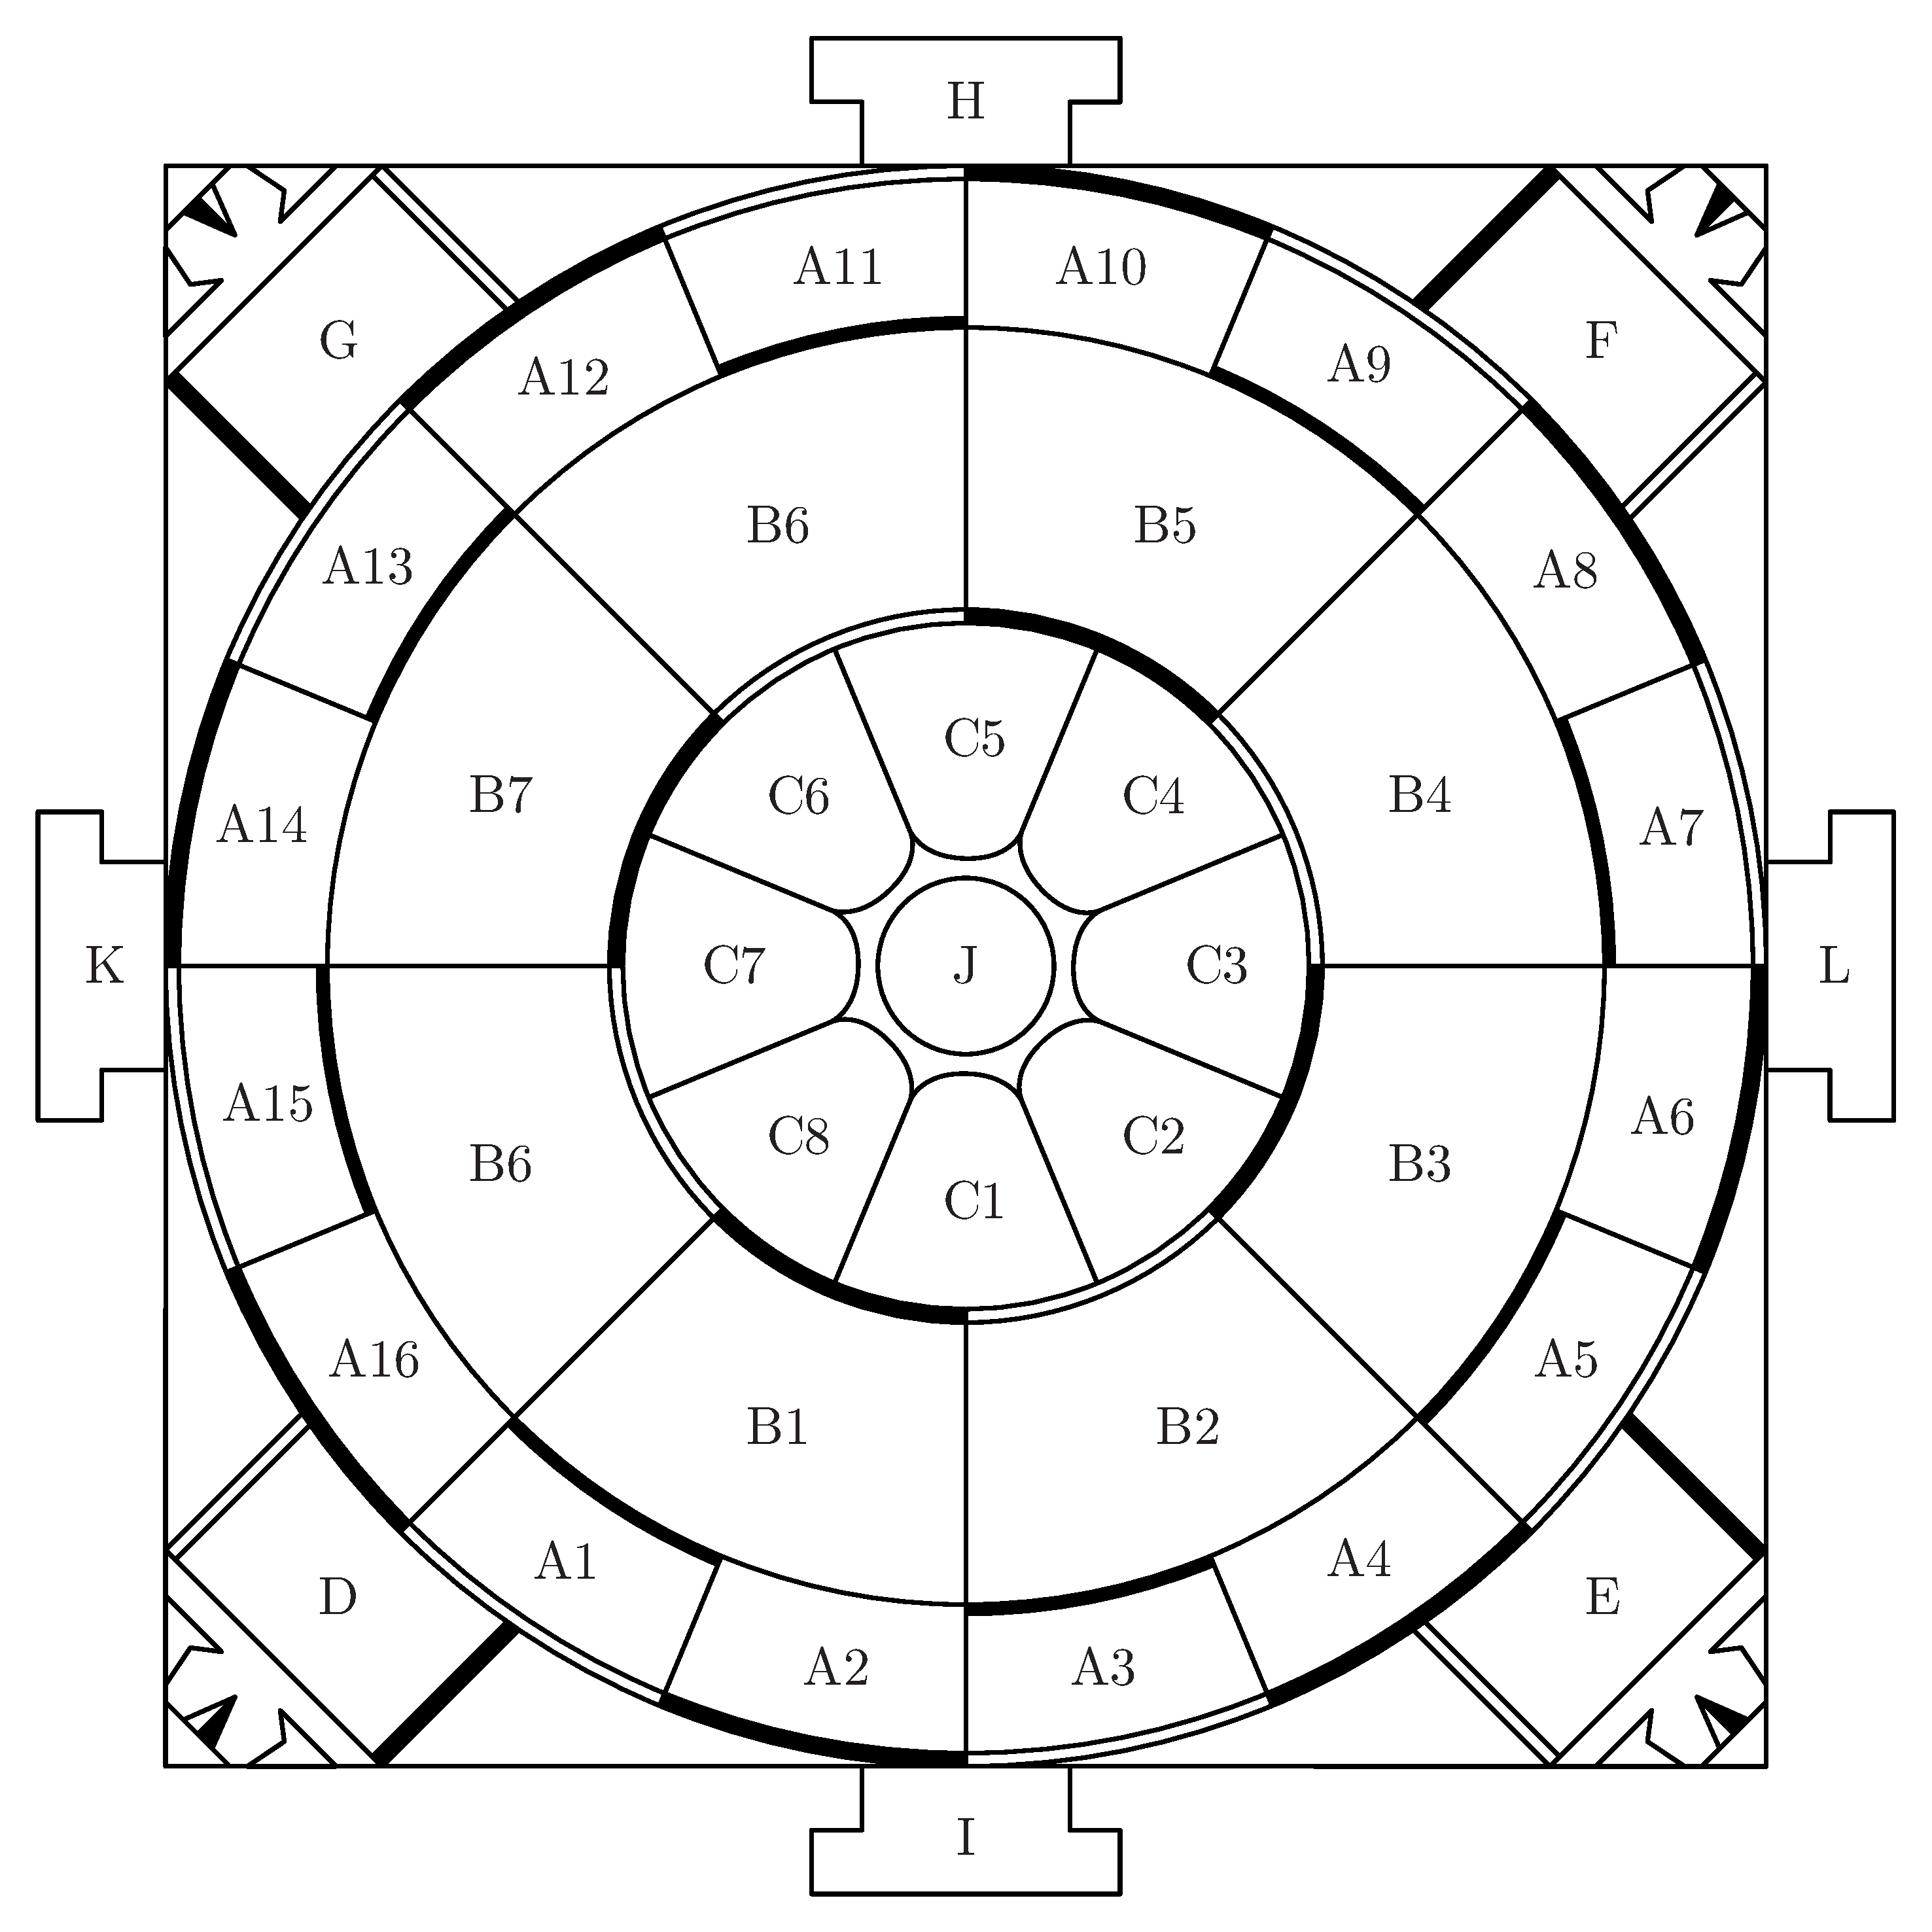
\includegraphics[scale = 0.4]{mandala-explain} }
\end{figure}

\begin{figure}
	\caption{原始國中手繪圖}
	\label{c}
	\centerline{ 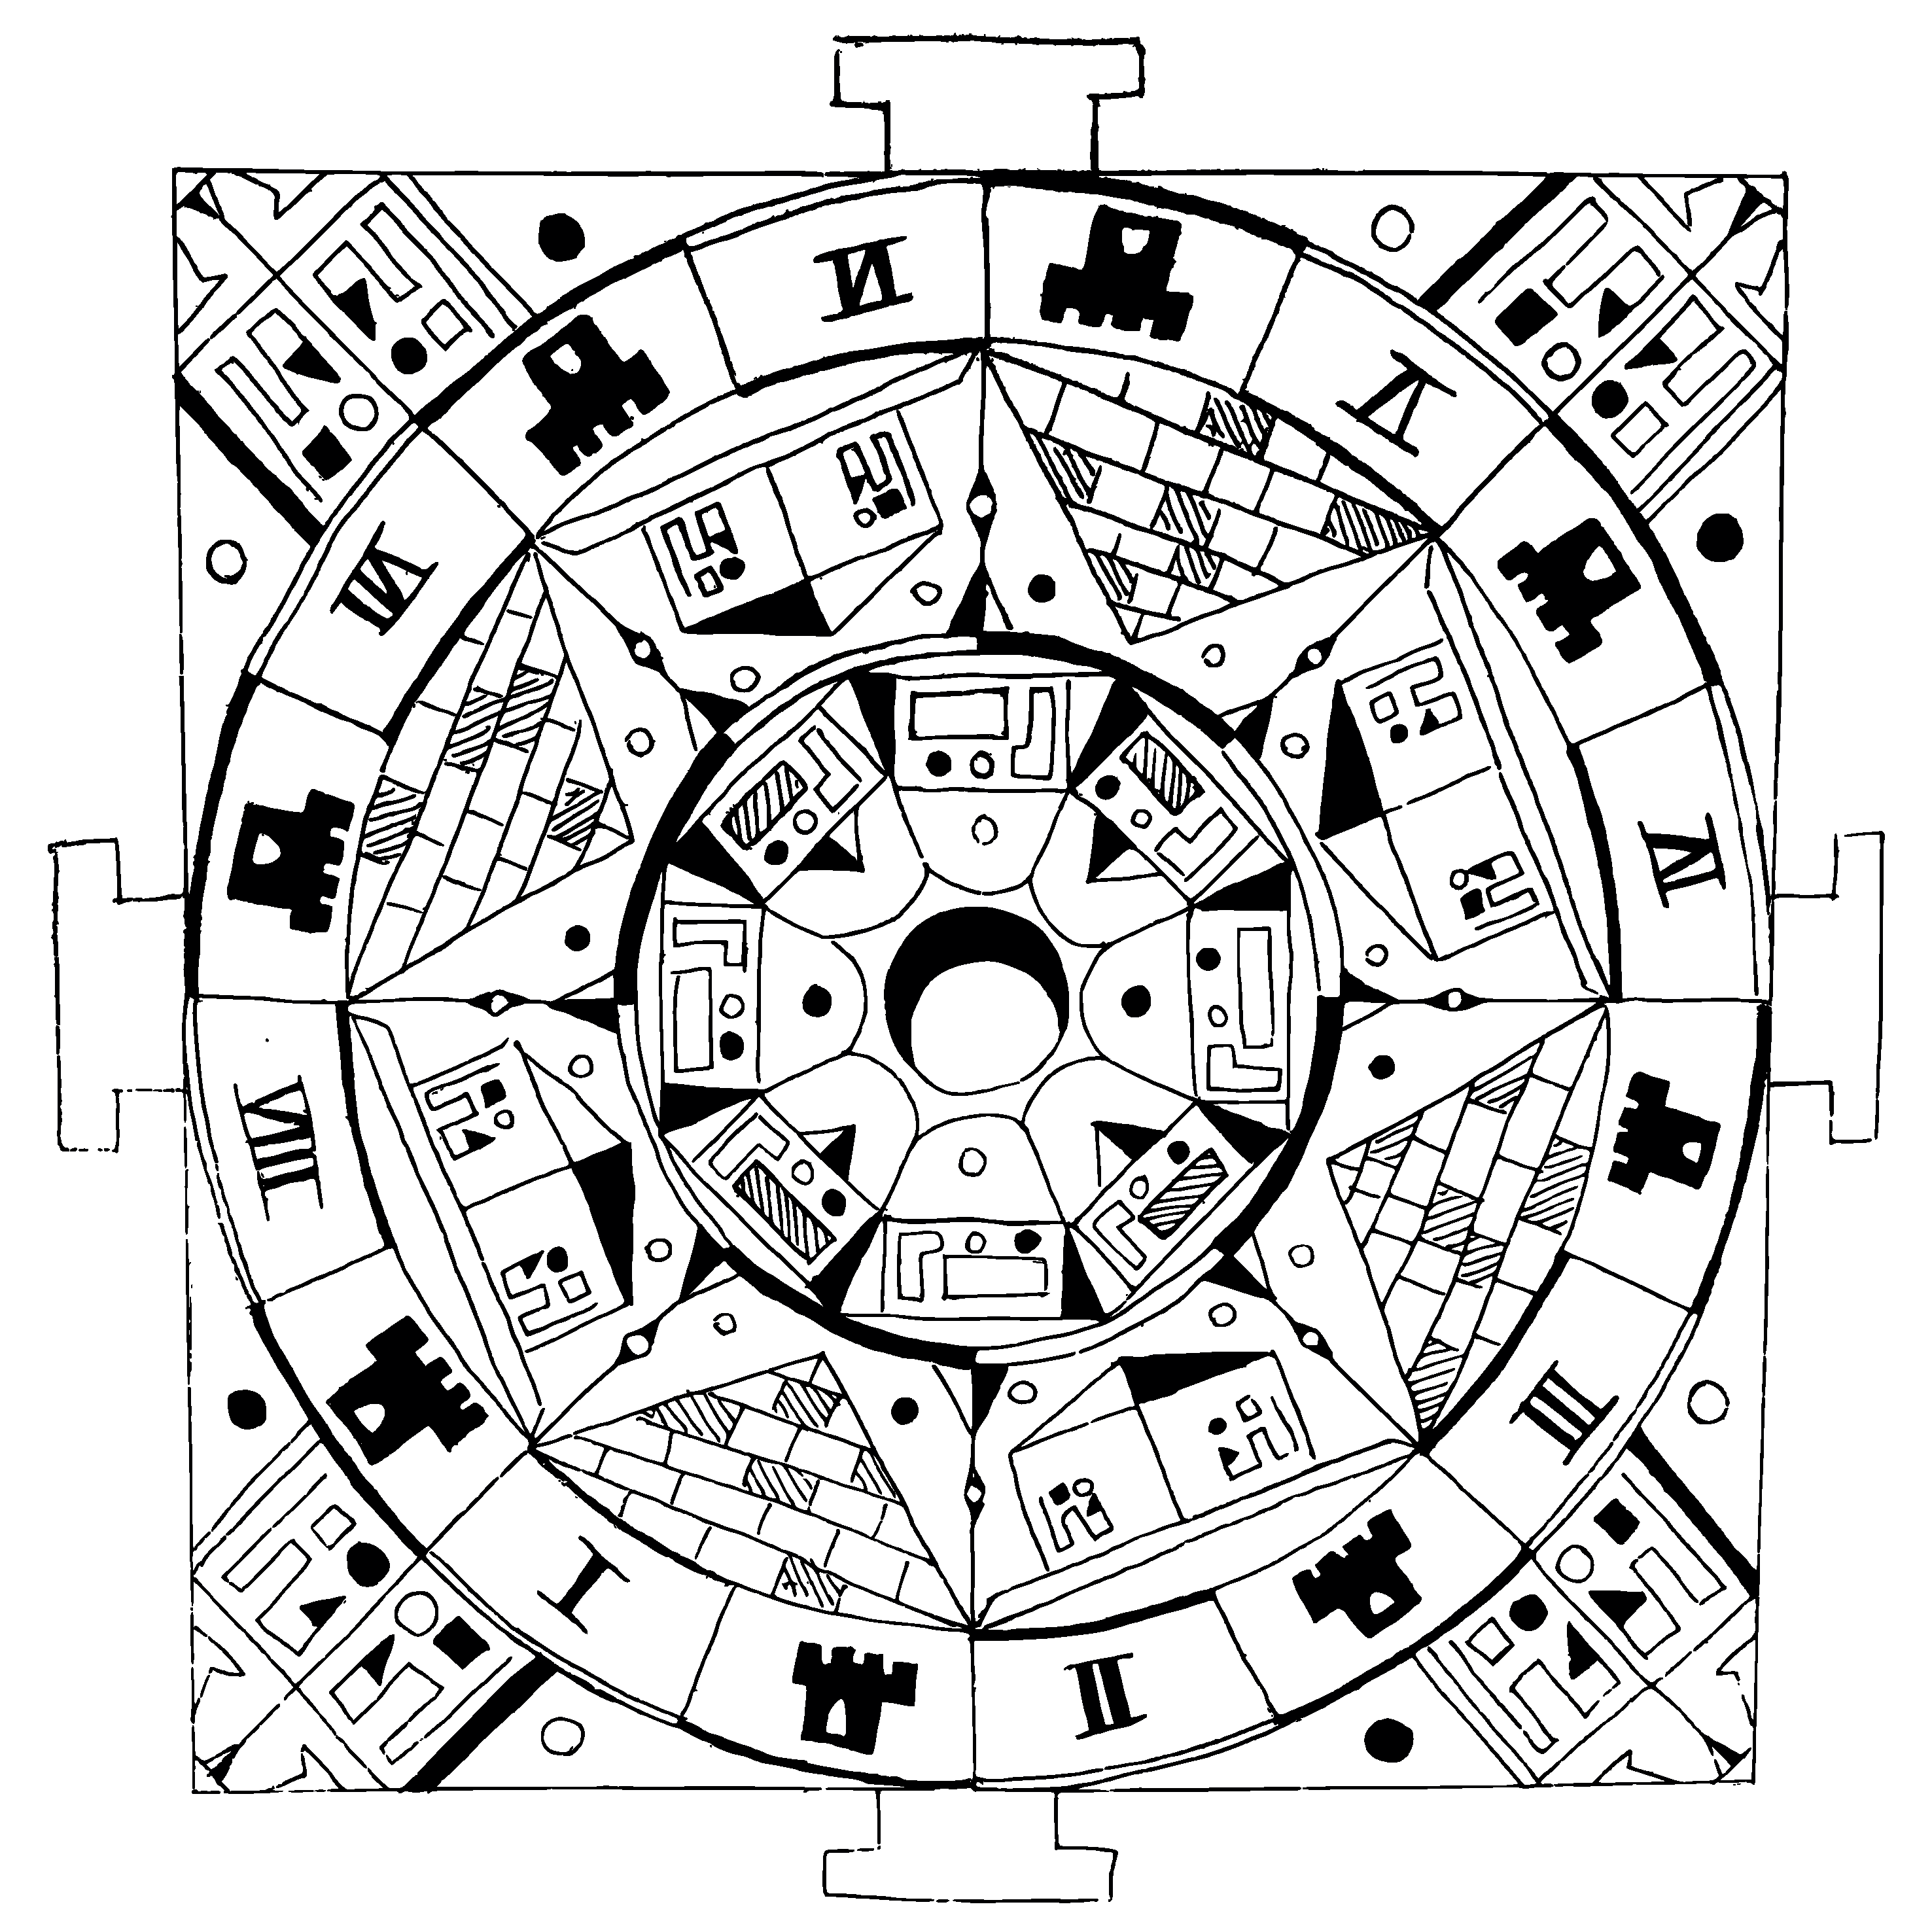
\includegraphics[scale = 0.4]{mandala-traced-01} }
\end{figure}

\end{document}
